\documentclass{beamer}

\usepackage[utf8]{inputenc}
\usepackage[danish]{babel}
\usepackage{tikz}
\definecolor{Plum}{rgb}{0.56, 0.27, 0.52}
\usetikzlibrary{arrows}
\usetikzlibrary{decorations.markings}
\graphicspath{{../imgs/}}

\usetheme{Ilmenau}
\usecolortheme{beaver}
\uselanguage{Danish}
\languagepath{Danish}
\usepackage{xcolor}

\newcommand{\unit}[1]{\ensuremath{\:\text{#1}}}
\newcommand{\pro}{\ensuremath{\unit{\%{}}}}
\graphicspath{{../imgs/}}

\expandafter\def\expandafter\insertshorttitle\expandafter{%
  \insertshorttitle\hfill%
  \insertframenumber\,/\,\inserttotalframenumber}

\title{DaLUKE}
\subtitle{
    Den Dansktalende Sprogmodel MED VIDEN
}
\author[Søren Holm, Asger Schultz]{Søren Winkel Holm, Asger Laurits Schultz}
\institute[DTU]{Danmarks Tekniske Universitet}
\date{7. juli 2021}

\begin{document}

\begin{frame}
    \titlepage
\end{frame}

%Kom hurtigt til resultater
%Relativt få slides
%Vis arbejde
%Understøt med figurer
%Evt demonstrerer med karaktereksempel
%Kort om anvendelse - meget efterspurgt i industrien
%Kom hurtigt frem til resultater
%Hav repræsentationen med

% Asger: Hvad er problemet? og Hvordan gik det?
% Søren: Hvordan vil vi løse det? og Hvad har vi lært?

\begin{frame}
    \frametitle{Fremlæggelsen}
    \footnotesize
    \tableofcontents
\end{frame}

\section{Hvad er problemet?}
\begin{frame}
    % 1
    \frametitle{Mangel på viden og lavresourcesprog}
    \begin{itemize}
        \item På trods af grammatisk korrekt og idiomatisk tekst ved modeller ikke, hvad de taler om\footnotemark
        \item Det forsøges løst med viden
        \item I lavresourcesprog fungerer det også som en udvidelse af datasæt
        \item Fx er den engelske Wikipedia $ \sim 40 $ gange større end den danske
    \end{itemize}
    \footnotetext{\url{https://www.technologyreview.com/2020/08/22/1007539/gpt3-openai-language-generator-artificial-intelligence-ai-opinion}}
\end{frame}

\begin{frame}
    % 1
    \frametitle{Navngiven entitetsgenkendelse (NER)}
    \begin{itemize}
        \item Mål: Finde strengt definerede verdslige objekter i et dokument
        \item Praktiske anvendelser som informationssøgning, spørgsmålsbesvarelse og anonymisering
    \end{itemize}
    \begin{example}
        "Cæsar marcherede mod Rom og trodsede dermed det romerske senat."\\
        "Cæsar": person\\
        "Rom": sted\\
        "det romerske senat": organisation
    \end{example}
\end{frame}

\tikzstyle{every picture}+=[remember picture]
\tikzstyle{every path}=[<->,shorten <=1pt]

\newcommand{\nw}[2]{
    \tikz[baseline=(#2.base), inner sep = 0pt]{\node (#2) {\underline{#1}};}
}

\section{Hvordan vil vi løse det?}
\begin{frame}
    % 2
    \frametitle{LUKE tilfører viden til sprogmodeller}
    \begin{columns}
        \column{0.5\textwidth}
        \begin{itemize}
            \item Transformer-opmærksomhed modellerer ord-kontekst
            \item<2-> LUKE [Yam+20] regner også opmærksomhed over \emph{navngivne entiteter}
        \end{itemize}
        \column{0.5\textwidth}
            \uncover<2->{
                \begin{tabular}{c|c}
                    Entitet       & ID\\\hline
                    $\vdots$      & $\vdots$\\
                    New York City & \texttt 5\\
                    Christian 4.  & \texttt 6\\
                    $\vdots$      & $\vdots$
                \end{tabular}
            }
    \end{columns}
    \begin{example}
        \footnotesize
        \only<1>{
            \nw{Fredag}{1} \nw{rykkede}{2} Syd- og Sønderjyllands \nw{Politi}{3} ud til Sønderborg \nw{Lufthavn}{4}.
            \begin{tikzpicture}[overlay]
                \path[->,blue!60,thick](1) edge [out=-90, in=-90] (2);
                \path[->,blue,very thick](3) edge [out=-90, in=-90] (4);
            \end{tikzpicture}
        }
        \only<2>{
            \nw{Fredag}{1} \nw{rykkede}{2} \nw{Syd- og Sønderjyllands Politi}{3} ud til \nw{Sønderborg Lufthavn}{4}.
            \begin{tikzpicture}[overlay]
                \path[->,blue!60,thick](1) edge [out=-90, in=-90] (2);
                \path[->,red, very thick](3) edge [out=-90, in=-90] (4);
            \end{tikzpicture}
        }
    \end{example}

\end{frame}

\begin{frame}
    % 3
    \frametitle{En prætrænet, frit tilgængelig DaLUKE}
    \begin{figure}[H]
        \centering
        \begin{tikzpicture}[shorten >=1pt,->,draw=black!90, scale=0.5, every node/.style={scale=0.5}]
\tikzstyle{every pin edge}=[<-,shorten <=1pt]
\tikzstyle{path} = [ultra thick]
\tikzstyle{neuron}=[circle,fill=black!25,minimum size=17pt,inner sep=0pt]

\tikzstyle{shared neuron}=[neuron, fill=purple!90];
\tikzstyle{word neuron}=[neuron, fill=blue!90];
\tikzstyle{entity neuron}=[neuron, fill=red!90];

\tikzstyle{annot} = [text width=10em, text centered]

\node[annot] (I) at (-2, 0) {\footnotesize Wikipediatekst med entiteter};

\node[word neuron] (T-W) at (0, 2) {};
\node[entity neuron] (T-E) at (0, -2) {};
\node[annot, above of=T-W, node distance=1 cm] {Ord-tokenizer};
\node[annot, below of=T-E, node distance=1 cm] {Entitetsordbog};

\path (I) edge (T-W);
\path (I) edge (T-E);

\node[word neuron] (E-W) at (4, 2) {};
\node[entity neuron] (E-E) at (4, -2) {};
\node[annot, above of=E-W, node distance=1 cm] {Ord-embeddings};
\node[annot, below of=E-E, node distance=1 cm] {Entetitsembeddings};

\path (T-W) edge (E-W);
\path (T-E) edge (E-E);

\node[annot] at (2, 2.25) {\footnotesize $m$ delord-ID'er};
\node[annot, text width=5em] at (2, -2) {\footnotesize $n$ entitets- og pos.-ID'er};

\node[rectangle, draw = black,
    text = white,
    align=center,
    fill = Plum,
    minimum width = 4cm,
    minimum height = 2cm
    ] (T) at (6,0) {Transformer:\\\(12\times\text{opmærksomhed}\)};

\path (E-W) edge (T);
\path (E-E) edge (T);

\node[annot, text width=4em] at (5.25, 1.5) {\footnotesize $\mathbf w_{1, \ldots, m}$};
\node[annot, text width=4em] at (5.25, -1.5) {\footnotesize $\mathbf e_{1, \ldots, n}$};

\node[annot, text width=1em] at (9,0) {\footnotesize
    $\begin{bmatrix}
    \textcolor{blue!90}{\mathbf x_1}     \\
    \textcolor{blue!90}{\vdots}  \\
    \textcolor{blue!90}{\mathbf x_{m}}   \\
    \textcolor{red!90}{\mathbf x_{m+1}} \\
    \textcolor{red!90}{\vdots}  \\
    \textcolor{red!90}{\mathbf x_{m + n}}
    \end{bmatrix}
    $
};
\path (T) edge (8.75, 0);

\node[annot, text width=4em] (F) at (11, 0) {Gæt skjulte ord og entiteter};
\path (9.75, 0) edge (F);
\end{tikzpicture}

    \end{figure}\noindent
    % \begin{itemize}
    %     \item Egen software
    %     \item Ingredienser
    %         \subitem Initialisér 
    %     \item Dansk Wikipedia giver entiteter
    %     \item Dansk BERT [Bot19] giver ord-transformer
    %     \item Diskriminerer mellem ord og entiteter i opmærksomhed
    % \end{itemize}
\end{frame}

\section{Hvordan gik det?}
\begin{frame}
    % 3
    \frametitle{NER på dansk}
    Primært datasæt: \emph{DaNE} med 5.512 annoterede sætninger, heraf $ \sim 10\pro $ til validering og $ \sim 10\pro $ til test
    \begin{columns}
        \column{0.45\textwidth}
        \begin{itemize}
            \item Fire kategorier: LOC, PER, ORG og MISC
            \item Hovedmodel: Prætrænet i 150 epoker og fine-tunet i 15.
            Opnår 82,9\pro\ med MISC og 85,2 uden -- andenplads på DaNLP's liste
        \end{itemize}
        \column{0.55\textwidth}
        \begin{figure}[H]
            \centering
            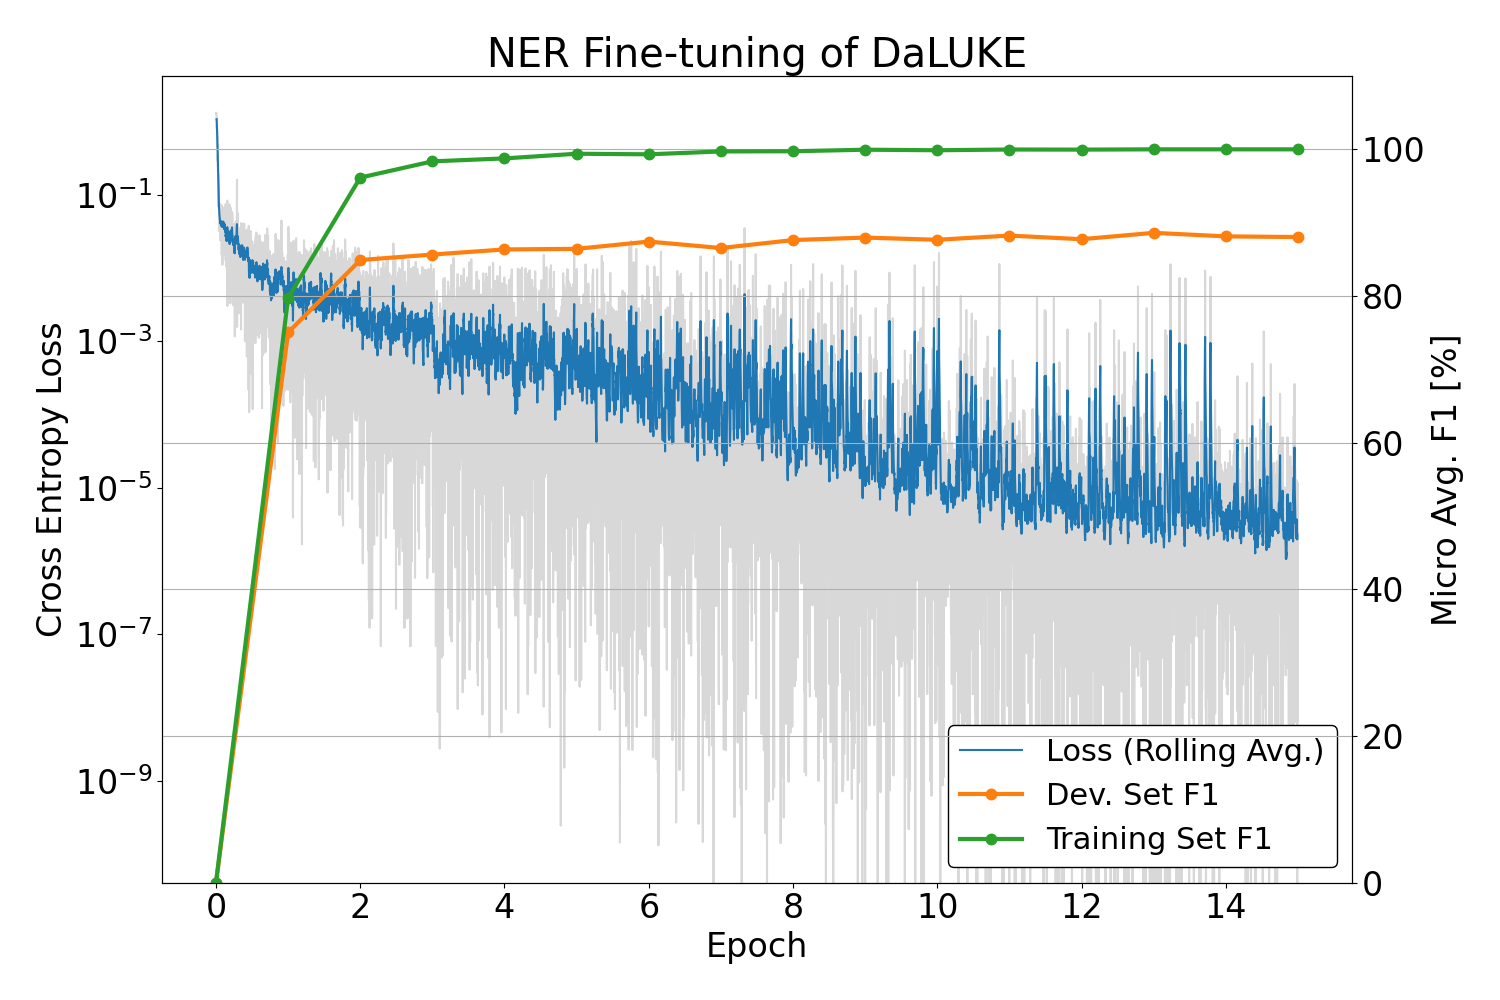
\includegraphics[width=\textwidth]{loss-fine}
        \end{figure}
    \end{columns}
\end{frame}

\begin{frame}
    % 3
    \frametitle{Entitetsbevidst selvopmærksomhed}
    \begin{columns}
        \column{0.6\textwidth}
        \begin{itemize}
            \item Transformerudvidelse, der modellerer entitets-entitets- og ord-entitets-forhold direkte
            \item LUKE bruger ikke entitetsbevidst selvopmærksomhed i prætræningen, men DaLUKE gør
            \item Bedre resultater dog påvist i diverse fine-tuningsopgaver
            \item Uden brug i prætræning falder fine-tuningsresultater med 2,8 procentpoint
        \end{itemize}
        \column{0.4\textwidth}
        
    \end{columns}
\end{frame}

\begin{frame}
    % 2
    \frametitle{Transferlæring}
    \begin{columns}
        \column{0.4\textwidth}
        \begin{itemize}
            \item Hvad hvis man ikke initialiserede fra da-BERT?
            \item Langt bedre præcision i prætræning - tyder på overfitting
            \item Fine-tuning ligger 11,4 procentpoint under baseline
            \item Transferlæring virker stabiliserende og regulariserende
        \end{itemize}
        \column{0.6\textwidth}
        \begin{figure}[H]
            \centering
            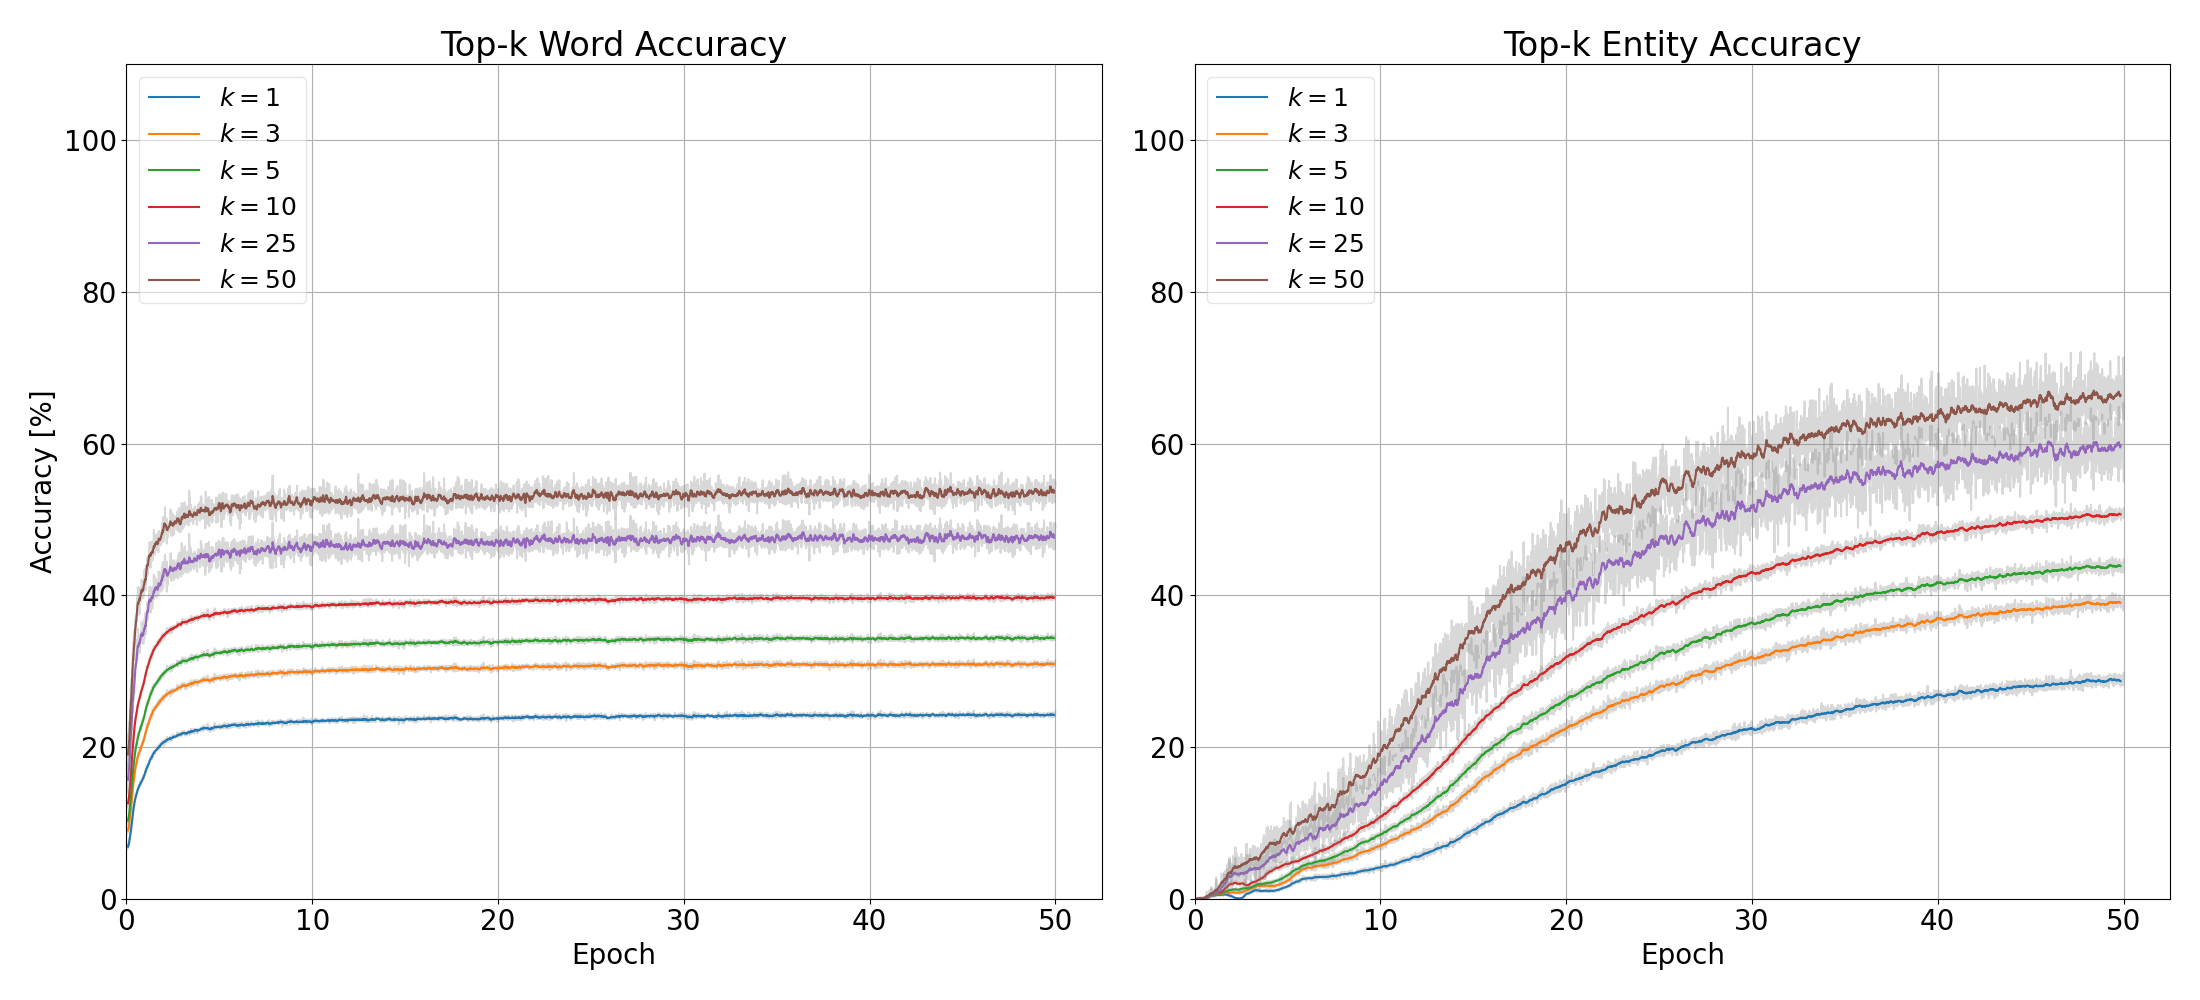
\includegraphics[width=.85\textwidth]{baseline-acc}
            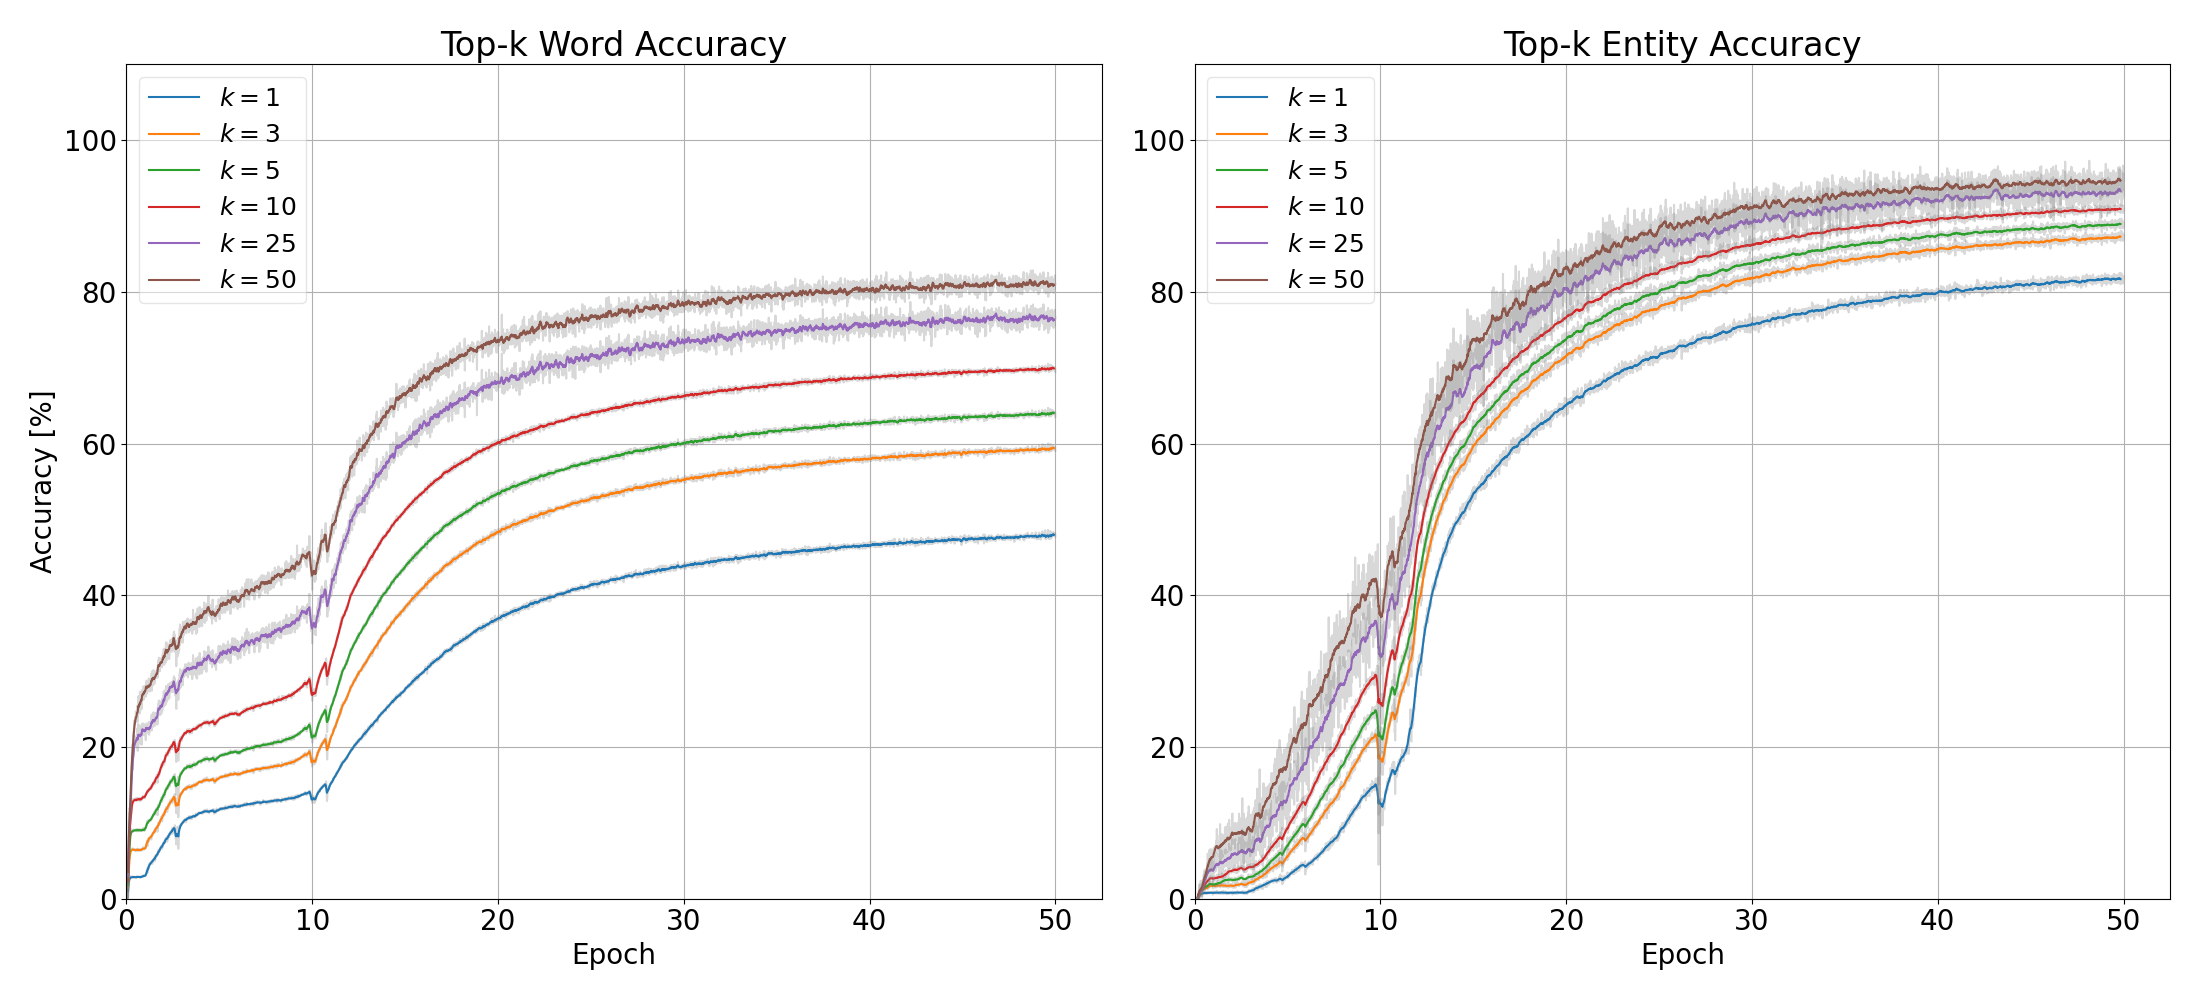
\includegraphics[width=.85\textwidth]{nobert-acc}
            \caption{Øverst: Baseline. Nederst: Ingen transferlæring}
        \end{figure}\noindent
    \end{columns}
\end{frame}

\begin{frame}
    % 2
    \frametitle{Datasætmodifikationer}
    \begin{itemize}
        \item Datasæt udvides med ekstra entiteter automatisk: $ 47\pro $ flere
        \item Uden dem fås 0,6 procentpoint højere; dog lille forskel ift. varians
        \item I LUKE beskæres entitetsordforrådet til de mest brugte. Hvilken effekt har det i DaLUKE?
        \item 0,2 procentpoint lavere med færre entiteter
    \end{itemize}
    \begin{example}
        "Arkæologi er studiet af tidligere tiders {\color{red}menneske}lige {\color{red}aktivitet}, primært gennem studiet af {\color<2>{blue}menneske}ts materielle levn. Langt det meste af al {\color<2>{blue}menneske}lig {\color{red}aktivitet} foregik, før vi lærte at skrive, så {\color<2>{blue}arkæologi} er den vigtigste metode til at studere ældre {\color<2>{blue}menneske}skabte samfund."
    \end{example}
\end{frame}

\section{Hvad har vi lært?}

\begin{frame}
    % 2
    \frametitle{NER-resultater er usikre}
    % Lille sample
    % RNG
    % Krydsvalidering
\end{frame}

\begin{frame}
    % 3
    \frametitle{Entiteter fanger sprogforståelse}
\end{frame}

\begin{frame}
    % 3
    \frametitle{Kontekst og viden i eksempler}
\end{frame}

\begin{frame}
    % 1
    \frametitle{Vejen til AI, der forstår dansk}
\end{frame}

\end{document}
